To study excited \cascade baryons the simulation of a sufficient number of signal events is needed.
For this study 1.5 million signal events were generated with the event generator EvtGen.
The reaction and decay tree selected for the simulation is shown in figure \ref{fig:eventgeneration_decaychannel}.
If not otherwise specified, the charged conjugate process is implicitly included in the following. 

\begin{figure}[htbp]
	\centering
			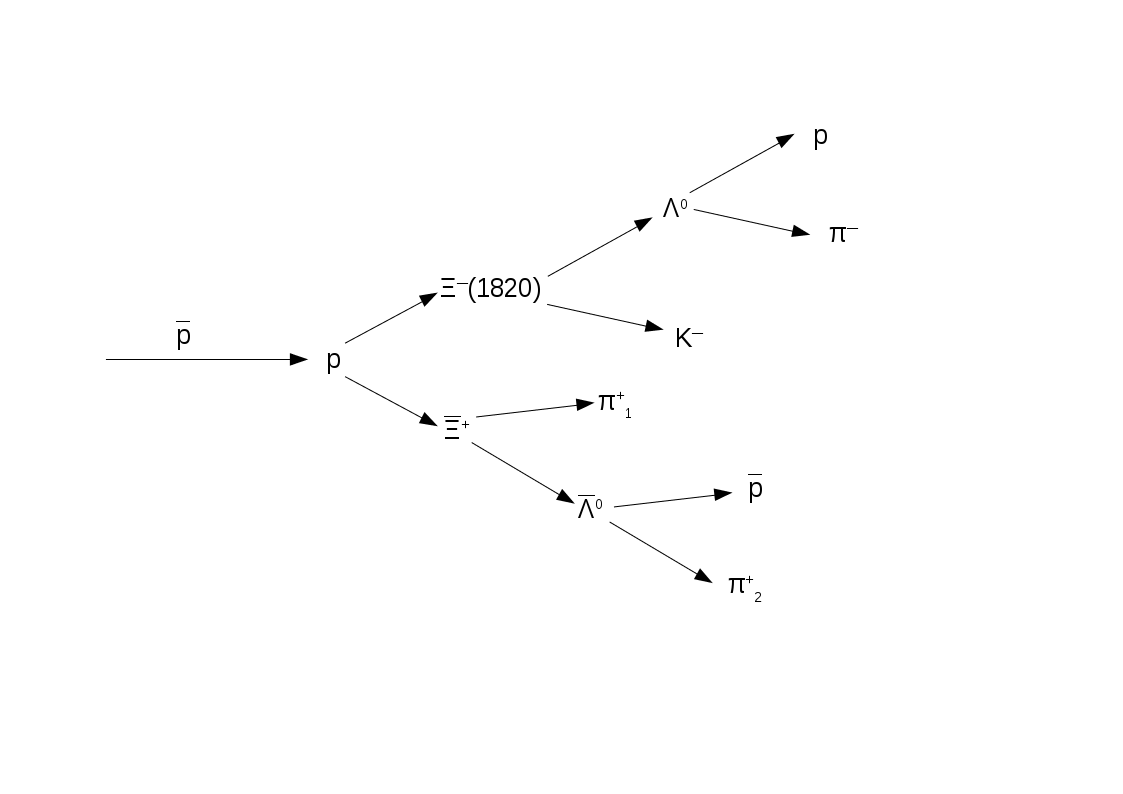
\includegraphics[width=1.00\textwidth]{./plots/DecayChannelXi1820.png}
	\caption{Reaction and decay tree selected for the simulation.}
	\label{fig:eventgeneration_decaychannel}
\end{figure}

For the charge conjugate channel another 1.5 million events were generated.
Table \ref{tab:eventgeneration_parameter} shows the parameters used for the event generation.

\begin{table}[tbp]
	\caption{Parameter for event generation}
	\label{tab:eventgeneration_parameter}
	\centering
	\begin{tabular}{ll}
		\hline
		Parameter & Value \\
		\hline
		\hline
		Beam momentum & 4.6 \massunit \\
		Production & PHSP \\
		Tracking & Ideal \\
		Particle ID & Ideal \\\hline
		 
	\end{tabular}
\end{table}

For the production reaction \pbarpSystem $\rightarrow$ \excitedcascade\anticascade the PHSP model, 
generating an isotropic angular distribution, was used,
because a more realistic treatment has not yet been implemented in EvtGen. 
This simplification does not affect the strategy used for this study.

The chosen beam momentum $p_{\bar{\mt{p}}} = 4.6\unit{GeV/c}$ corresponds to a center-of-mass energy 
of 100 MeV above the production threshold of \excitedcascade and \anticascade.
The production cross section is expected to be of the same order ($\sim \mu\mt{b}$) as for ground 
state \cascade production in \pbarpSystem $\rightarrow$ \cascade\anticascade \cite{PANDAphysics2009}.
This expectation is based on ground state and excited state single strange hyperons production data in \pbarpSystem collisions \cite{CERN}.
\\
\vspace{11pt} 

The used software versions for PandaRoot and the external software package is listed in table \ref{tab:eventgeneration_software} 

\begin{table}[tb]
	\centering
	\caption{Used software versions}
	\label{tab:eventgeneration_software}
	\begin{tabular}{ll}
		\hline
		Software & Version \\
		\hline
		\hline
		FairSoft & mar15\\
		FairRoot & v-15.03a \\
		PandaRoot & trunk revision 28555 \\
		Geant & 3\\
		Genfit & 1\\\hline
			 
	\end{tabular}
\end{table}


The missing \excitedcascade was defined in the evt.pdl file. 
How the particle is added is shown in the code snippet \ref{lst:eventgeneration_evtpdl}.
The properties of \excitedcascade are listed in table \ref{tab:eventgeneration_Xivalues}.

\begin{lstlisting}[caption={snippet from evt.pdl}\label{lst:eventgeneration_evtpdl}, captionpos=t,breaklines=true]
add  p Particle Xi(1820)- 23314 1.8230000e+00 2.4000000e-02 2.0000000e-01 -3 3 0.0000000e+00 23314
add  p Particle anti-Xi(1820)+ -23314 1.8230000e+00 2.4000000e-02 2.0000000e-01 3 3 0.0000000e+00 -23314
\end{lstlisting}

\begin{table}[htbp]
	\centering
	\caption{Properties of \excitedcascade and \excitedanticascade. The values are taken from \cite{PDG}}
	\label{tab:eventgeneration_Xivalues}
	\begin{tabular}{lllllll}
		\hline
		Particle & J & I & P & Charge & Mass  & Width \\
		\hline
		\hline
		&&&&&&\\
		\excitedcascade & $\frac{3}{2}$ & $\frac{1}{2}$ & ($-1$) & ($-1$) & ($1.823 \pm 5$)\massunit & ($0.024 \pm 6) $ GeV \\
		\excitedanticascade & $\frac{3}{2}$ & $\frac{1}{2}$ & ($-1$) & 1 & ($1.823 \pm 5$)\massunit & ($0.024 \pm 6) $ GeV\\
		\hline
		  
	\end{tabular}
\end{table}

The generated transverse momentum against the longitudinal momentum for \lam, \alam, \anticascade and \excitedcascade is 
presented in figure \ref{fig:MC_lambda0_pt_vs_pz}% -- \ref{fig:MC_xi_pt_vs_pz}.\\


\begin{figure}
	\subfigure[\lam]{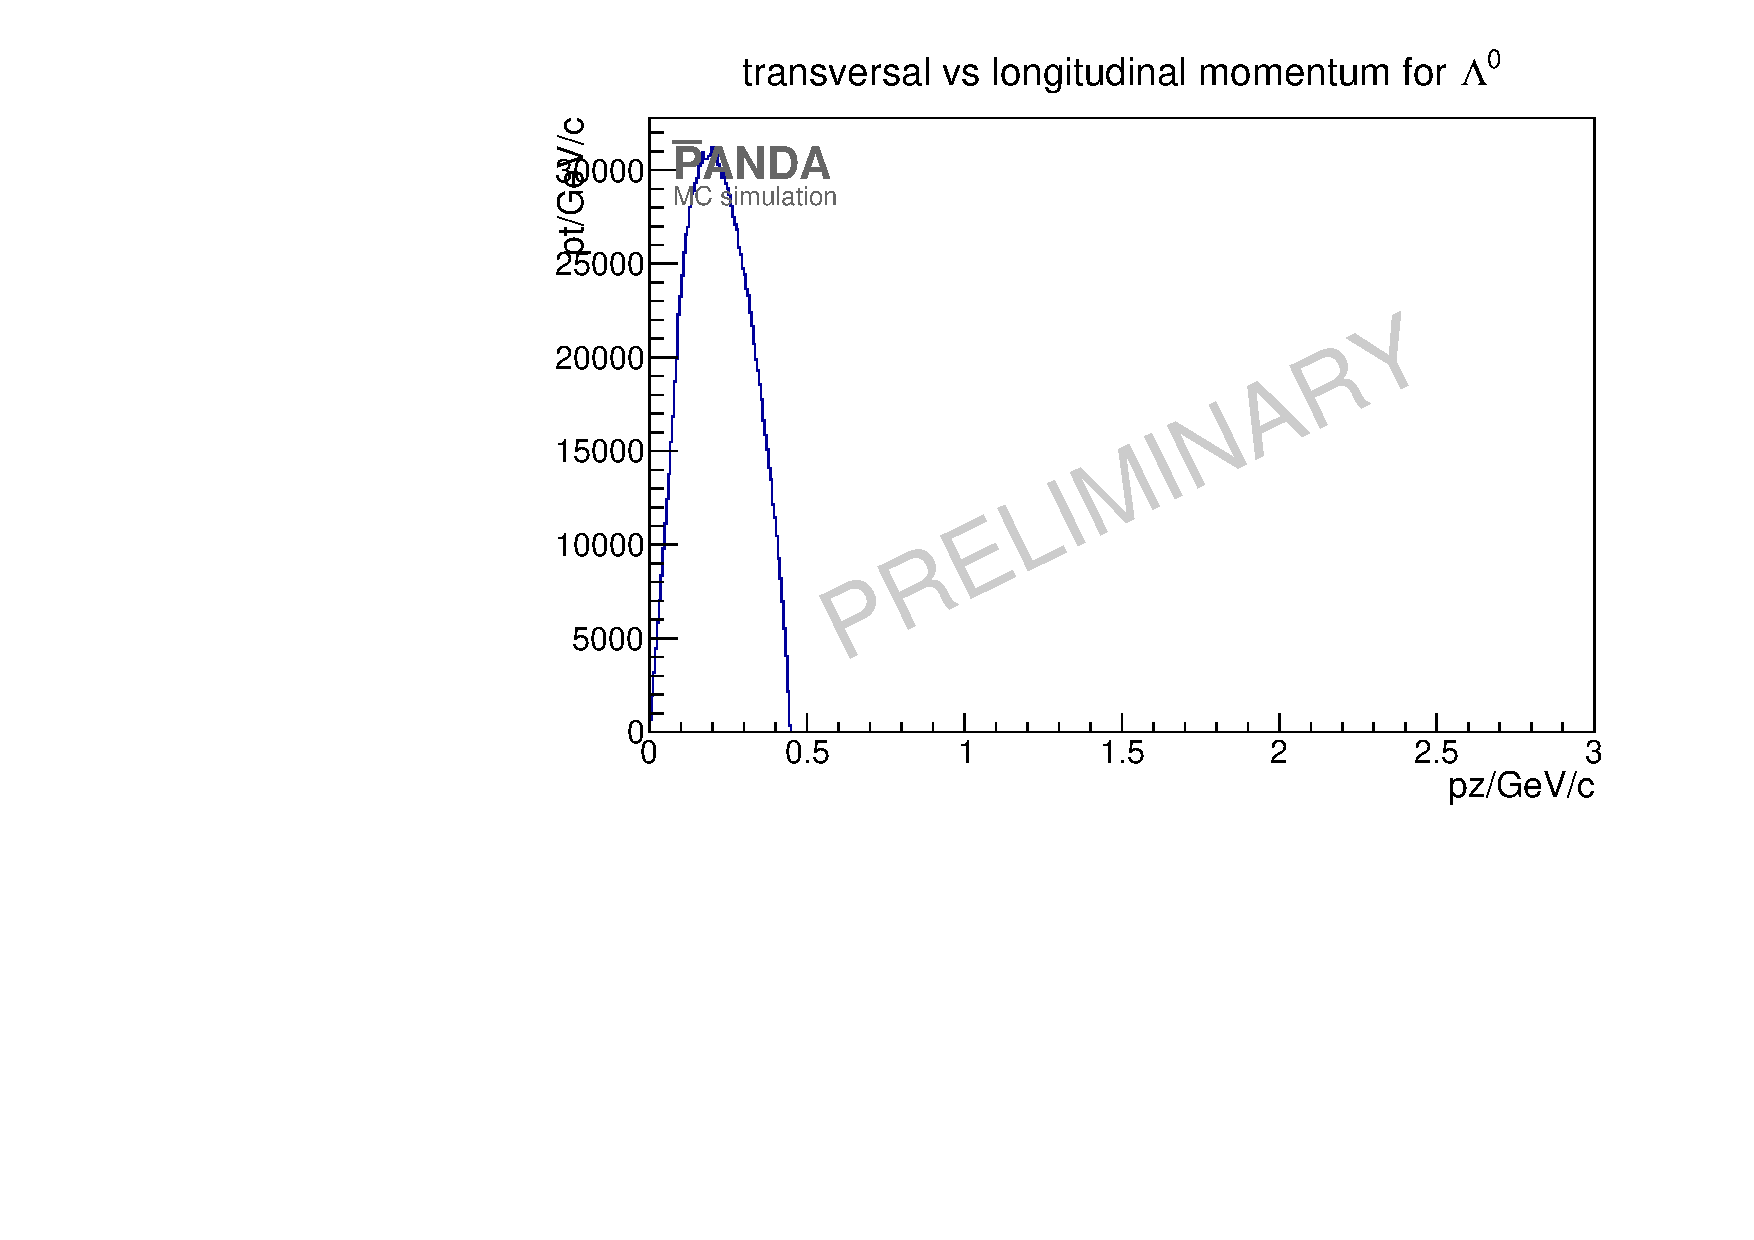
\includegraphics[width=0.49\textwidth]{./plots/lambda0/Lambda0_MC_pt_vs_pz.pdf}}
	\subfigure[\alam]{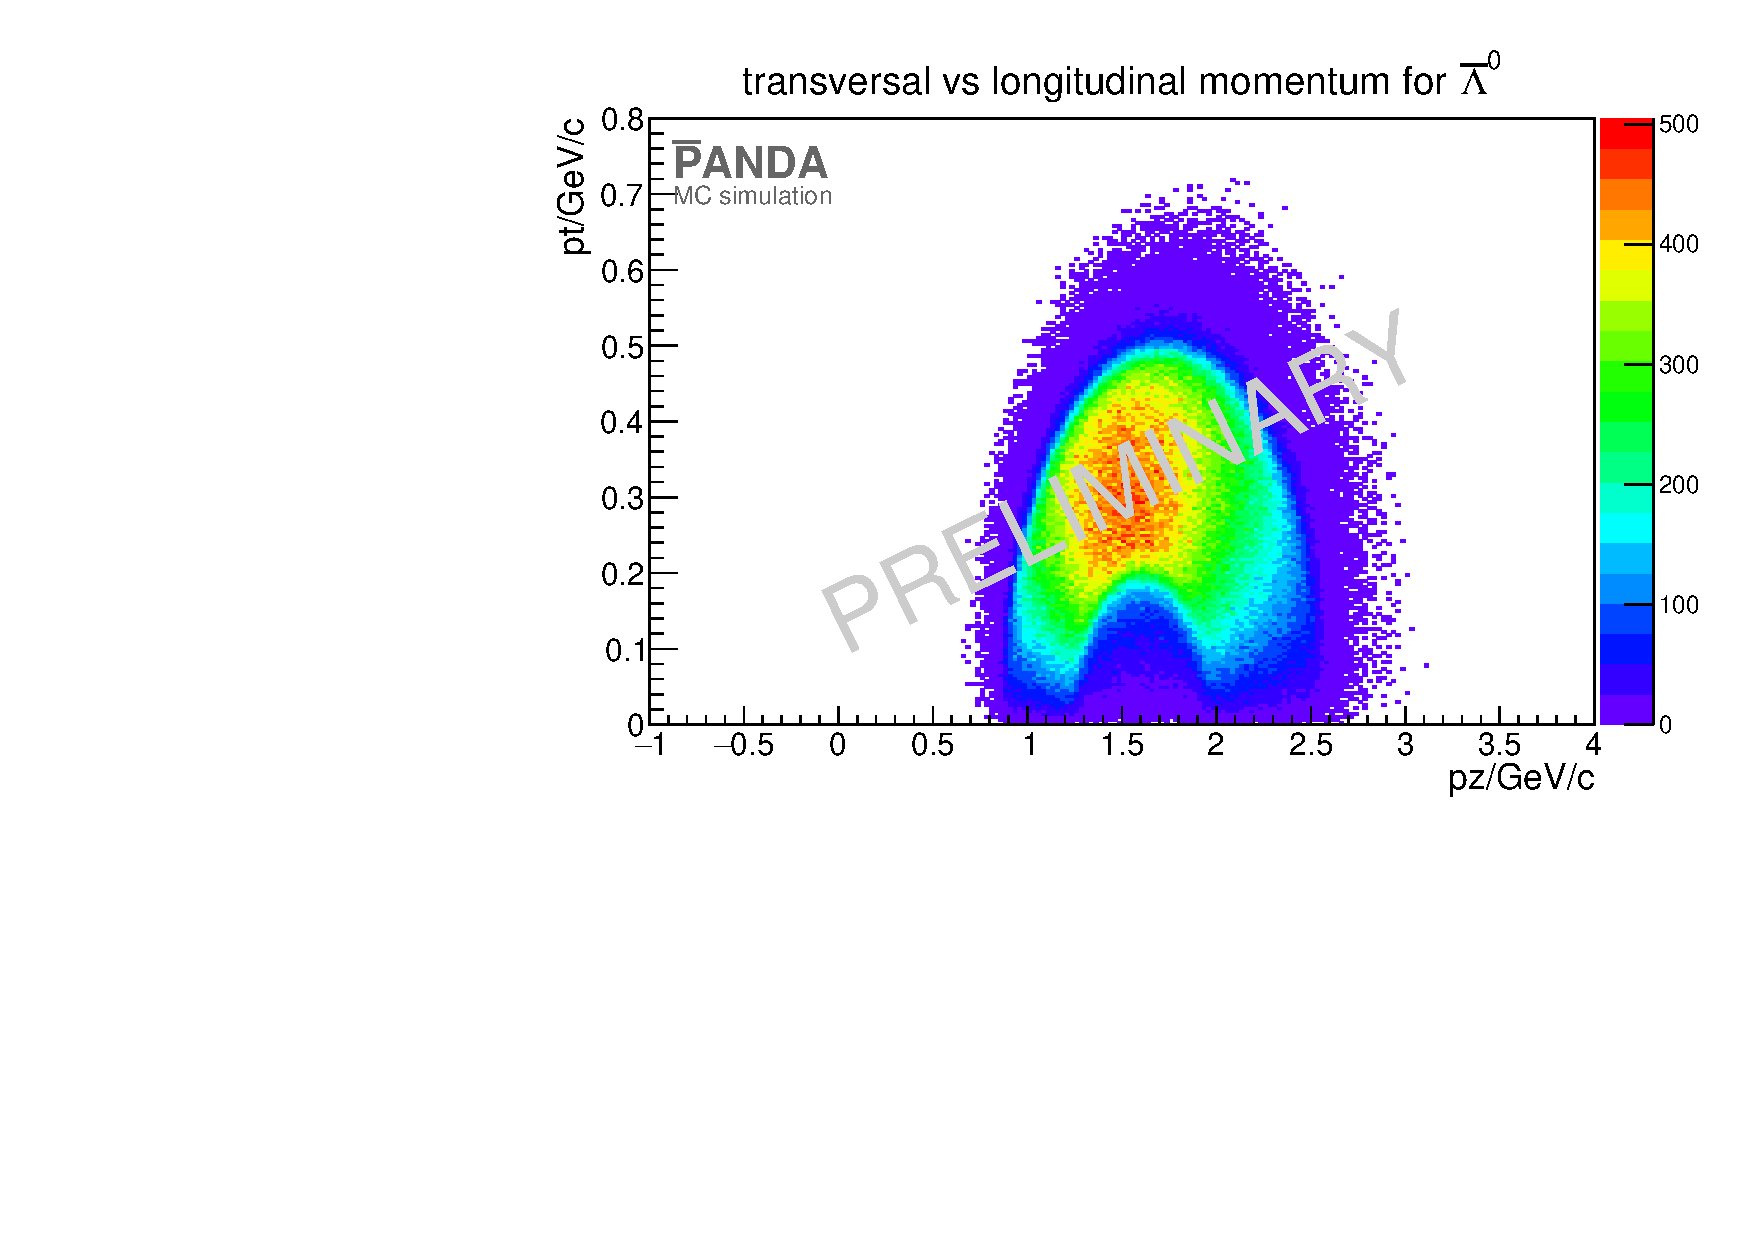
\includegraphics[width=0.49\textwidth]{./plots/antilambda0/AntiLambda0_MC_pt_vs_pz.pdf}}
	\caption{\propose Figure a) shows the transverse momentum on the y axis against the longitudinal momentum on the x axis for \lam. Figure b) 
			shows the same distribution for \alam.}
	\label{fig:MC_lambda0_pt_vs_pz}
\end{figure}


\begin{figure}
	\subfigure[\anticascade]{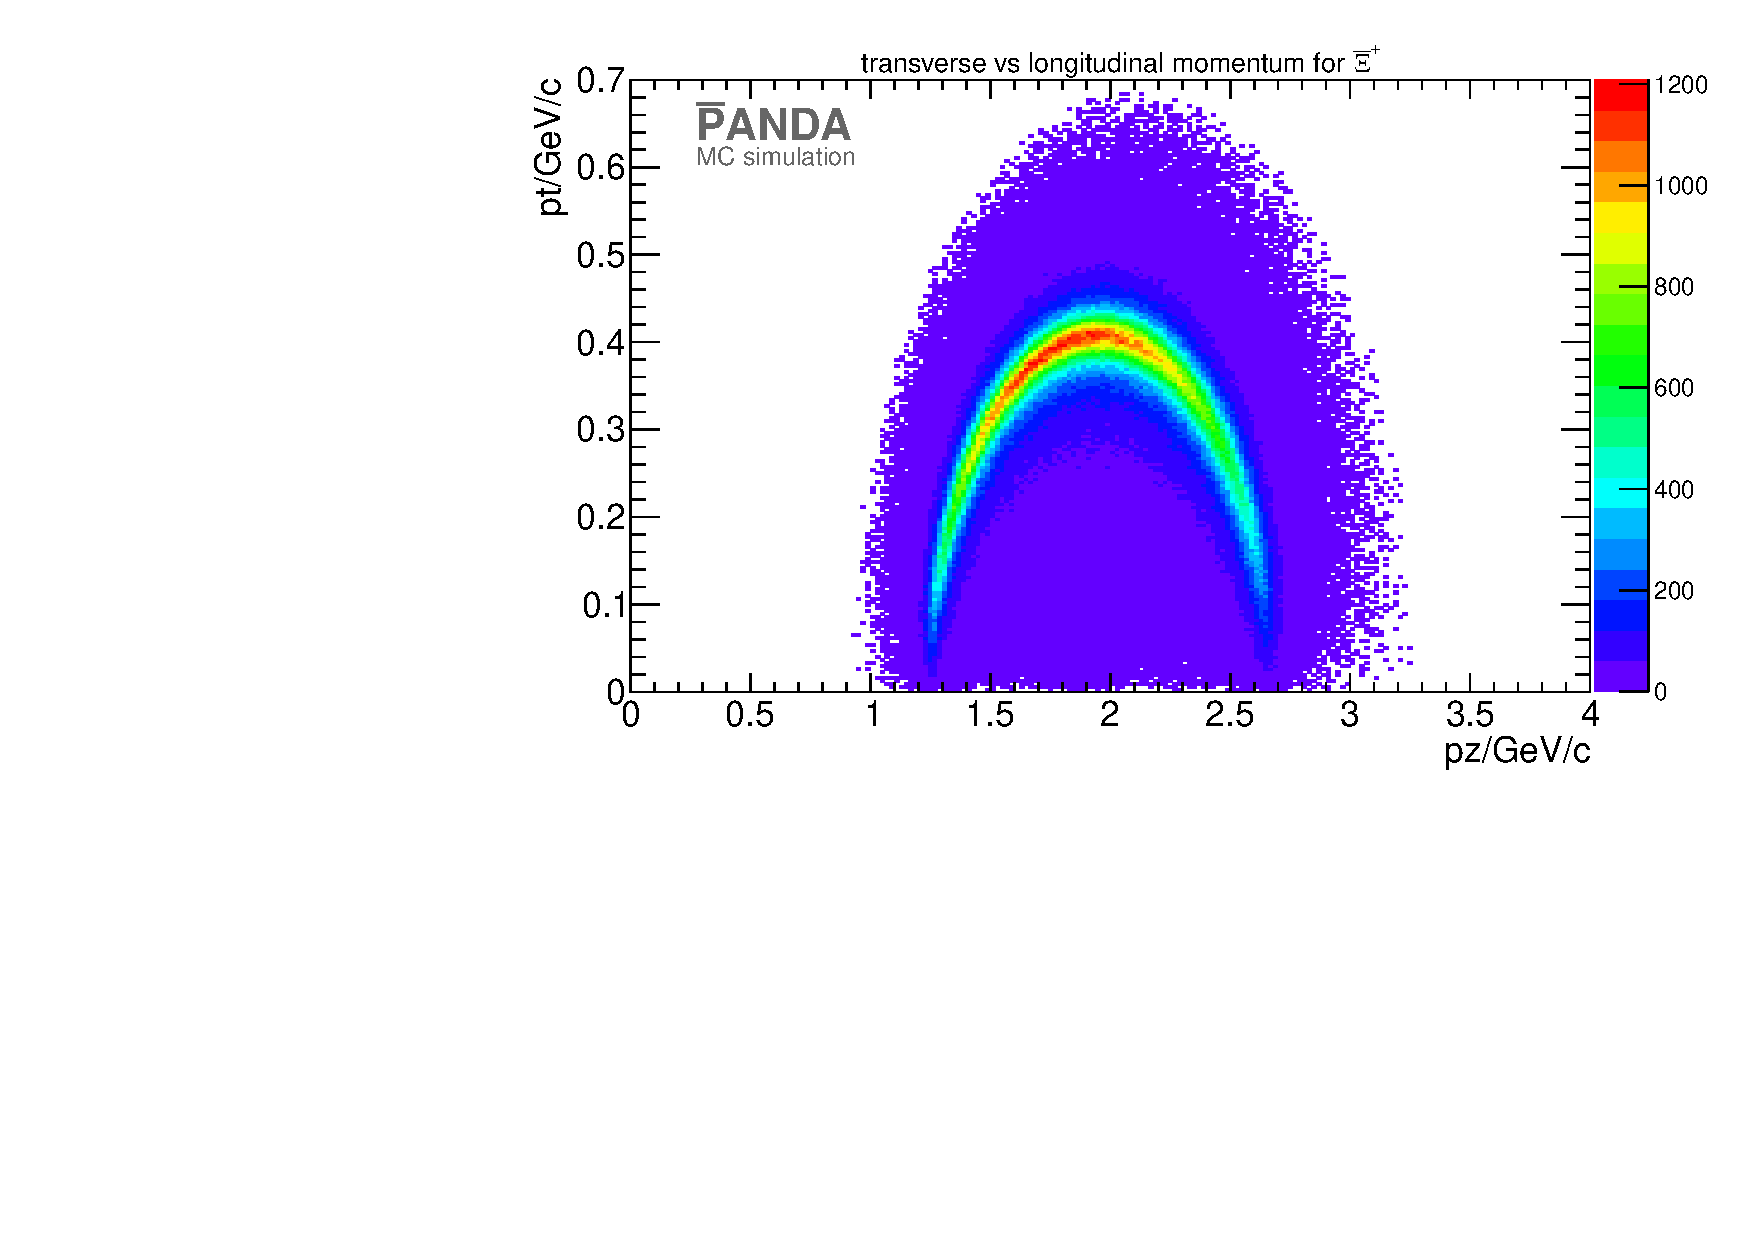
\includegraphics[width=0.49\textwidth]{./plots/Xi/XiPlus_MC_pt_vs_pz.pdf}}
	\subfigure[\excitedcascade]{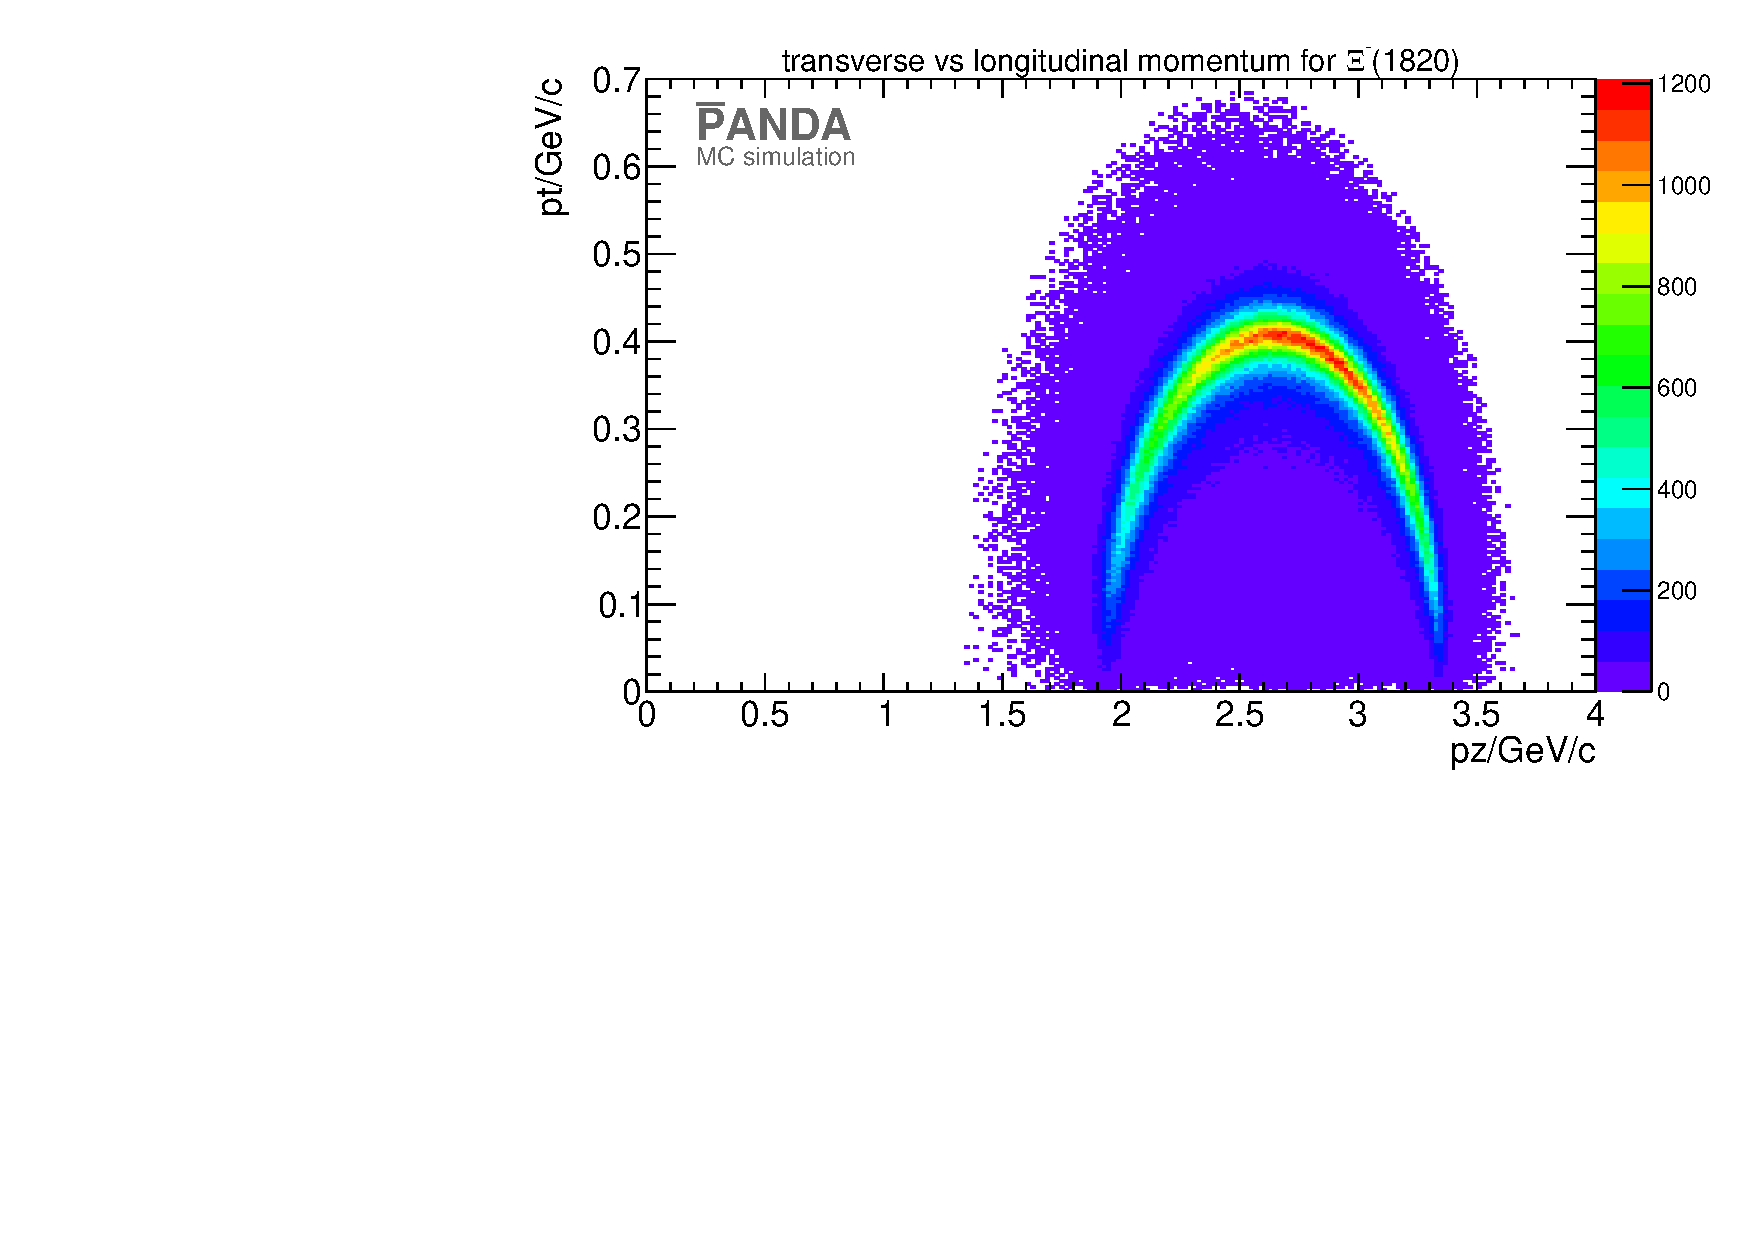
\includegraphics[width=0.49\textwidth]{./plots/Xi1820/XiMinus1820_MC_pt_vs_pz.pdf}}
	\caption{\propose Figure a) shows transverse against the longitudinal momentum distribution for \anticascade. Figure b) 
			transverse versus longitudinal momentum distribution for \excitedcascade.}
	\label{fig:MC_xi_pt_vs_pz}
\end{figure}

Figure \ref{fig:eventgeneration_Dalitz} shows the Dalitz plot for the \lam, \kminus and \anticascade final states for 
the channel \pbarpSystem $\rightarrow$ \excitedcascade \anticascade. 

\begin{figure}
	\centering
	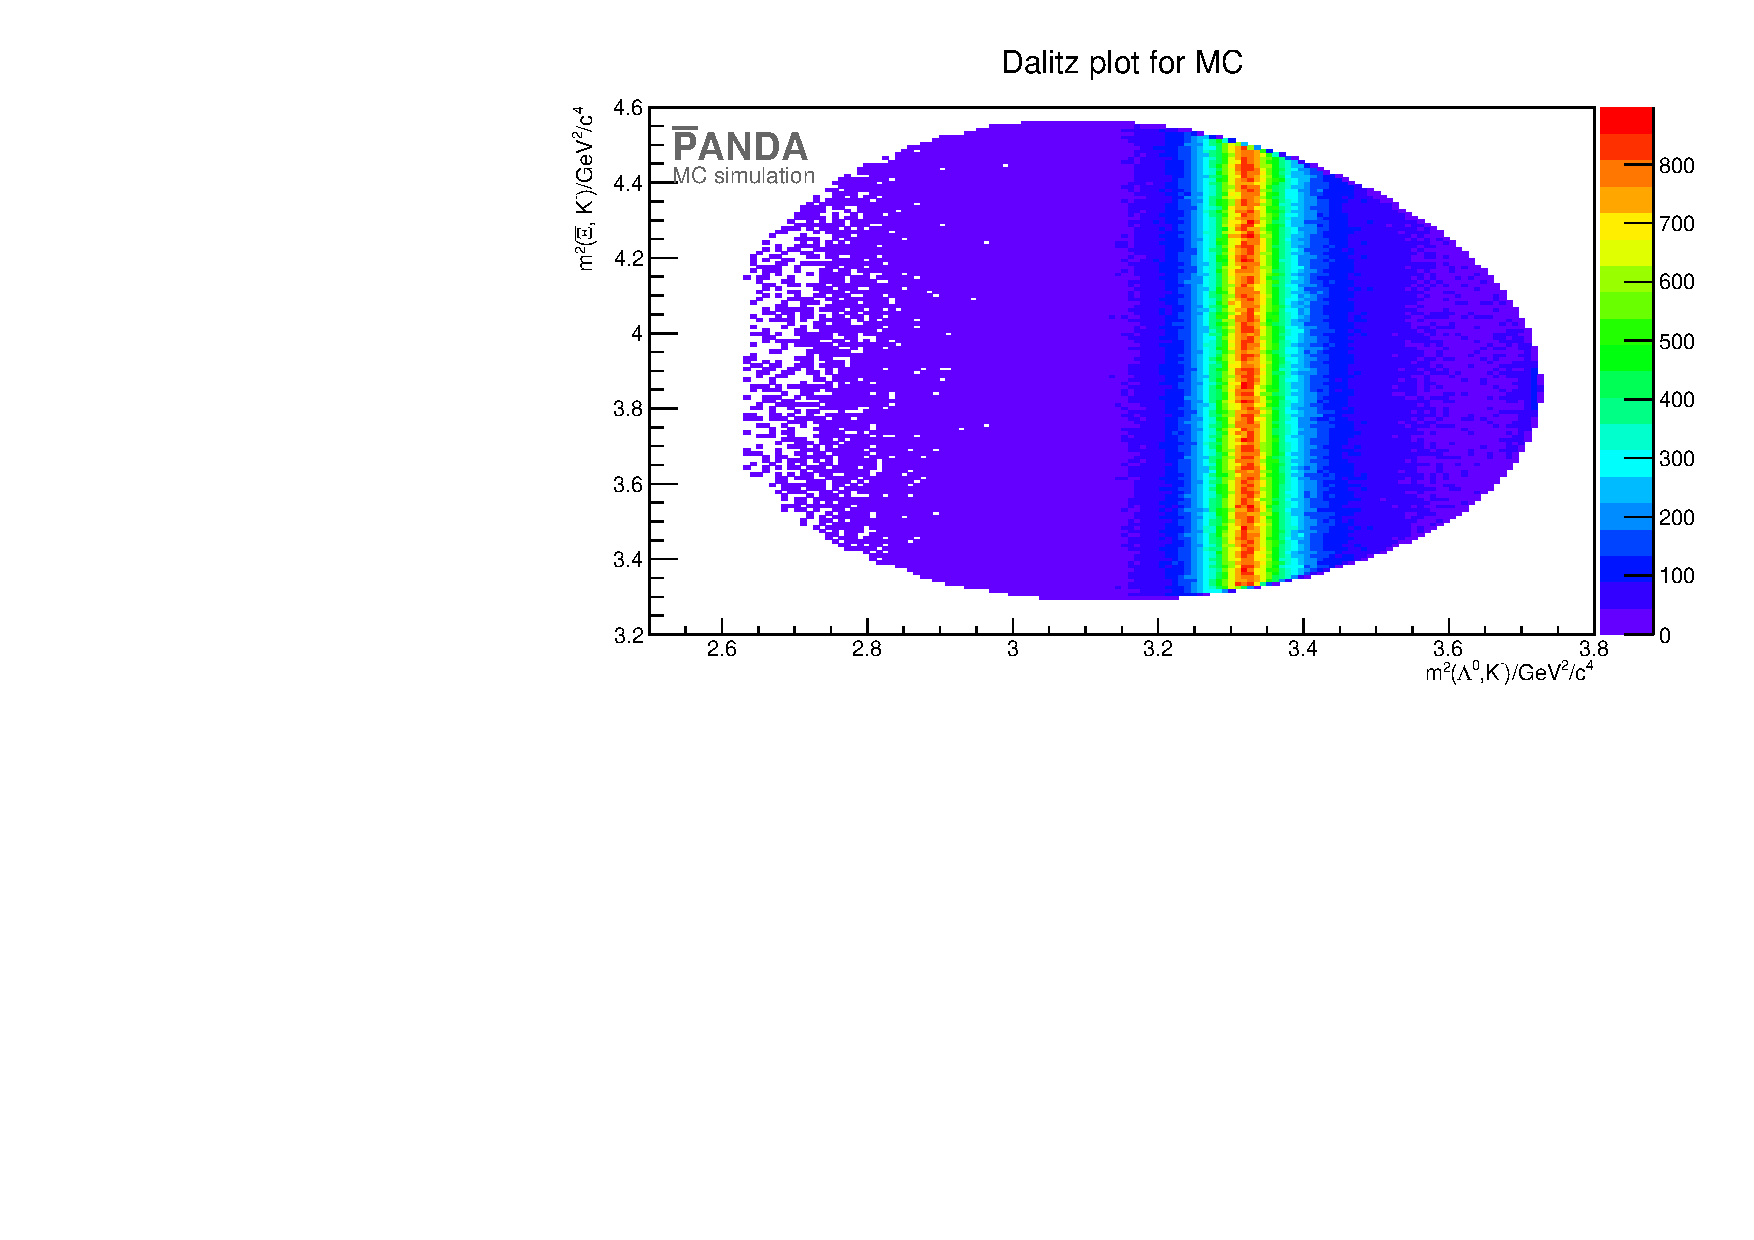
\includegraphics[width=0.6\textwidth]{./plots/Dalitzplot_MC.pdf}
	\caption{\propose Dalitz plot for simulation. On x axis is the mass square of \lam  and \kminus and on the y axis there is the mass square of \anticascade and \kminus}
	\label{fig:eventgeneration_Dalitz}
\end{figure}

